\section{Markets for a Self-Incentivizing Network}
\label{sec:designs}
We set out to design a market interface that any router could expose and users could interact with multiple markets.
We wanted to allow different users with their own objectives to be able to buy guaruntees of packet carriage but also change their reservations to increase their own percieved utility.

In the rest of the section, we introduce a first simple market to achieve these goals and then evaluate its performance with simulated users.
This intial design has high overhead and our current simulated users have the ability to change their utility for the worse because of market races with other users. We quantify this phenomena with a worst case "evil user," and finally propose a new multi-resolution market that addresses these problems.

%\begin{itemize}
%
%\item Let anybody contribute capacity
%
%\item Allow users with different utility functions to interact (flow completion time vs.~jitter)
%
%\item Allow users to buy guarantees (and not get swindled)
%
%\end{itemize}

\subsection{Simple Market Design}
Our market is composed of consecutive time slots in which a single packet can be delivered. Users are able to buy the rights to deliver a packet at a given time slot for a reserve price set by the market. Once a slot is owned by a user, they have the right to send a packet on the link at that time if they can deliver a packet to the router before that time. They can also add an offer to the slot to re-sell it to another user if they pay the offer price. Figure \ref{f:simple_market} gives the basic market layout.

can simulate multiple users with different objectives

\subsubsection{Flow completion time user}
This user type has a set number of packets $n$ it would like to send as soon as possible. It tries to maximize the utility function $U= -t - c$, where $t$ is the flow completion time and $c$ is the total amount paid for slots. In practice, this user checks the market to see if any of its slots have been sold and buys the $n$ slots that maximize its utility function. Once slots have been purchased, this user sets the price of each slot it owns to be \$.01 more than the loss of utility if they did not own that slot and had to buy another one.

\begin{figure}
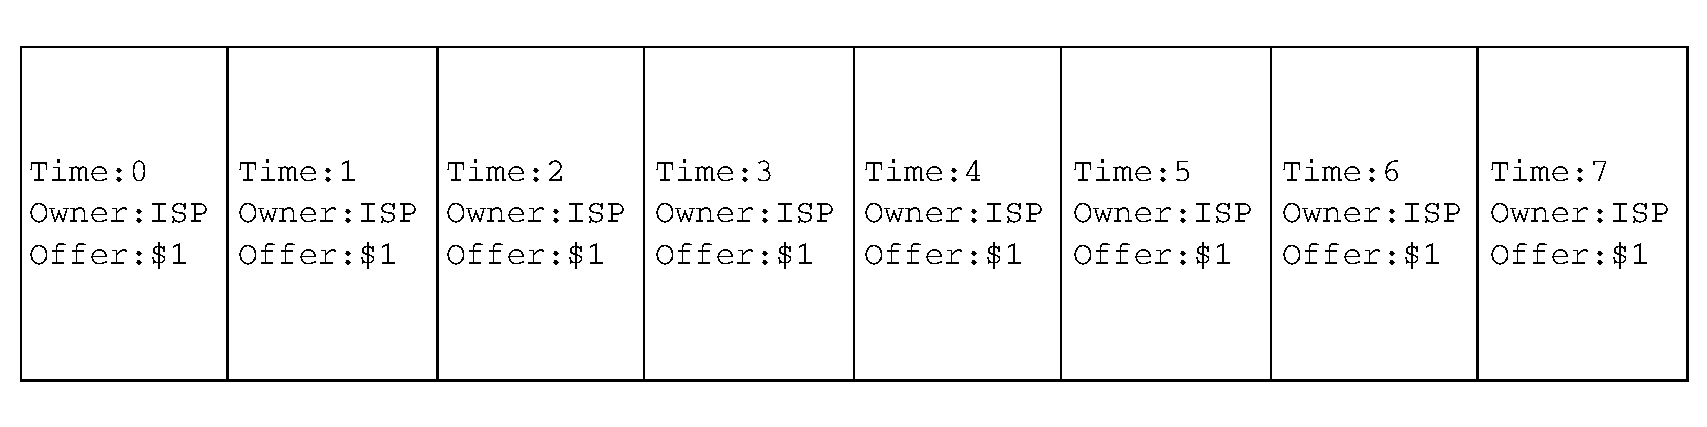
\includegraphics[width=\columnwidth]{diagrams/simple_market.pdf}
\caption{Simple market sample state. User A owns the first two time slots and has an offer of \$2.01 for each. User B owns the next two slots and has not put up an offer to sell them. User C owns slot at time 6 and has posted an offer of \$10 to sell it. ISP owns remaining slots with an offer of \$1 for each.}
\label{f:simple_market}
\end{figure}

\subsection{Simple Market Evaluation}

Simulation experiments to test whether the one-layer market has each desired property?

Measure outcome quality (vs.~SRTF or other optimal), \# of roundtrips

\begin{figure}
%\vspace{\baselineskip}
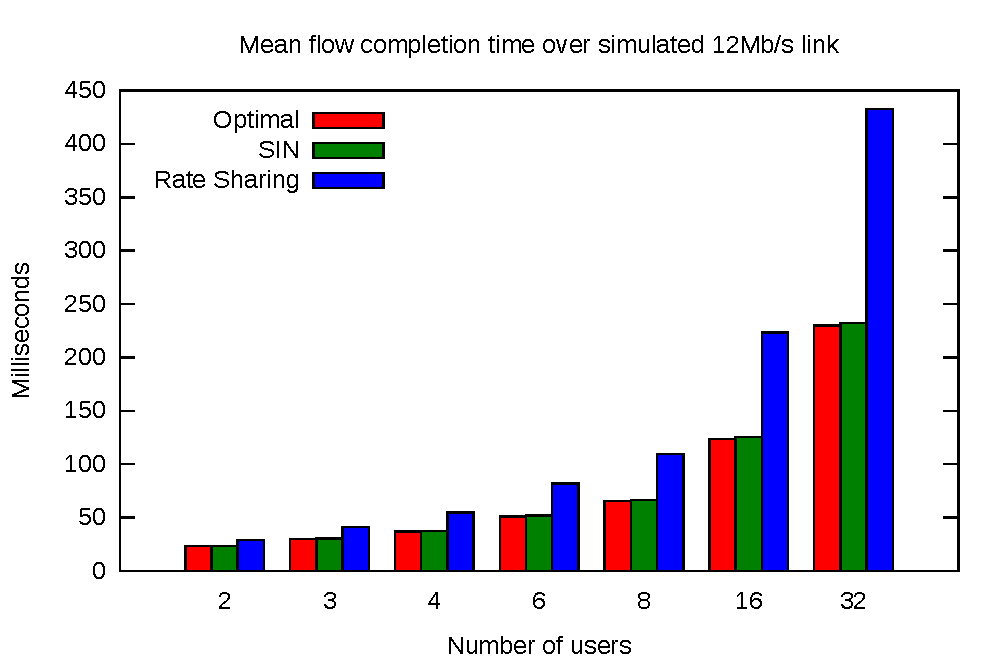
\includegraphics[width=\columnwidth]{plots/delay_over_srtf.pdf}
\caption{todo}
\label{f:delay_over_srtf}
\end{figure}

We simulated the results of running a market in practice with flow completion time users that would arrive at time $t$ had a known number of packets $n$ they wanted to send.
Figure~\ref{f:delay_over_srtf} shows the result of running the simulation with 2 to 10 concurrent users, all trying to minimize their flow completion time for the cheapest cost.
We compare with a round robin scheme, which is the ideal equillibrium of mutliple TCP flows and a FIFO queued router (TODO cite).
In our simulations, there are a varying number of users with a flow start time chosen from a uniform random distribution between 0 and 9 with flow lengths chosen from a uniform random distribution between 1 and 10. We compare to the allocation of packets to times that minimizes the queued time for each flow: shortest remaining time first scheduling (TODO cite).

We find that bots in our market almost always converge on an allocation that is equivalent to the optimal shortest remaining time first schedule when there is a small number of users. Larger numbers of users are less likely to achieve a perfectly optimal solution, but the excess queuing delay over the optimal SRTF solution remains extremely low with a large number of users: less than 1\% overhead in all of our evaluations.

\subsubsection{User Disappointment}
Unfortunately, in this scheme it is possible that a user would have had a higher utility at the end if it refused to put offers on its slots once it recieved them.
This is possible because a flow completion time user bases its offer prices on the price of a replacement slot, but that slot can be purchased and their offer can be matched before they can re-price their offer.
This leads to a phenomena we call Disappointment, which when a user puts offers on slots it owns expecting to only increase their overall utility function but instead reduce it.
While this does happen sometimes in our simulations (TODO maybe figure for this), a user normally increases their utility when they list a slot.
However, this Disappointment can be arbitrarily bad in the case of a hypothesized evil user: whose objective is to reduce the final utilityof another user.
\subsubsection{Evil User}
An evil user could maximally reduce the utility of a flow completion time user for the cheapest cost by buying the cheapest slot that that user has for sale, and then buying the next $m$ slots after the last packet of the flow completion time user without putting up offers. Unless the flow completion time can move earlier, this reduces the utility function of the flow completion time user by ... TODO need example with reserve prices I think. Possbily diagram.

problem: exposure problem, evil user

\subsubsection{Communication overhead}

\begin{figure}
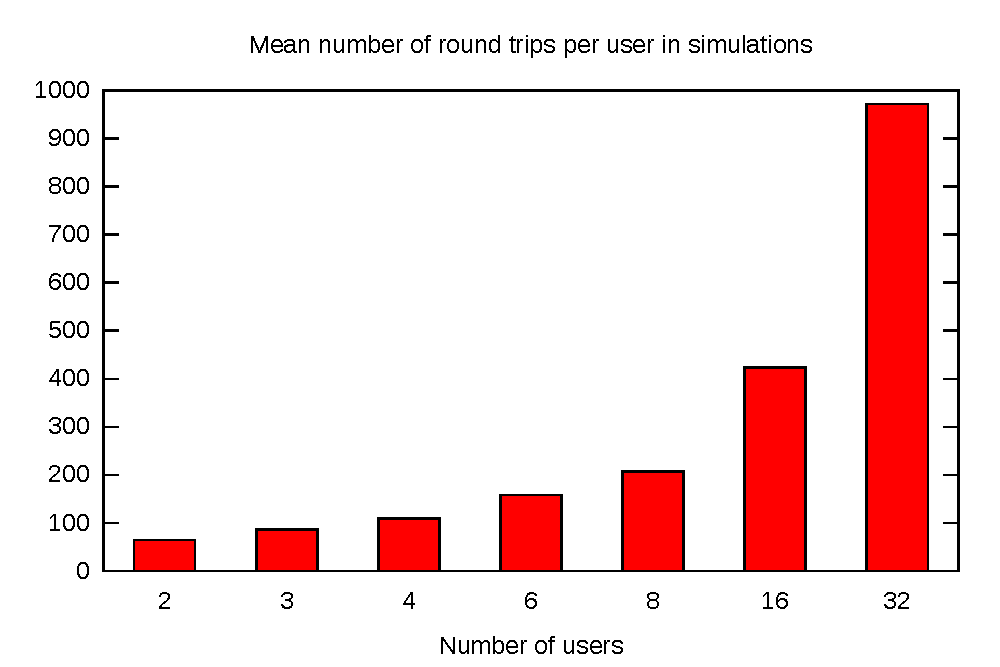
\includegraphics[width=\columnwidth]{plots/num_roundtrips.pdf}
\caption{todo}
\label{f:num_roundtrips}
\end{figure}

Another disadvantage of the simple market is that it can take a long time to converge on a solution where no user wants to buy more slots. In simulation flow completion time users would buy back and forth from each other many times, making small price adjustments throughout. The number of round trips each user performed is showin in Figure~\ref{f:num_roundtrips}. As more users concurrently access the market, the more roundtrips were required to reach a stable solution.


the problems we encountered with the simple market led us to our current design:
\subsection{Multi-Layer Market Design}

Sketch of multi-layer design
